\documentclass{article}
\usepackage{graphicx} % Required for inserting images
\usepackage{geometry}
\usepackage {ctex}
\usepackage{biblatex}  
\addbibresource{ref.bib}
\geometry{a4paper,scale=0.8}
\usepackage{amsmath}
\numberwithin{figure}{section}
\numberwithin{equation}{section}
\usepackage{multirow}
\numberwithin{table}{section}
\usepackage{booktabs}
\usepackage{array}
\usepackage[colorlinks,
            linkcolor=blue,
            anchorcolor=blue,
            citecolor=blue]{hyperref}

\title{PDE SIR}
\author{王乾宇}
\date{\today}

\begin{document}
\maketitle
\begin{abstract}
  老师我已完成部分模型搭建的工作(代码见\href{https://github.com/Aziliza/PDE_SIR}{github}),使用的方案二\ref{Solution}。在将真实数据带入求解事遇到了如下问题(具体见\ref{problem}),应该对年龄和时间分别选择哪个时间单位?比如在这个方程中,$a,t$的单位应该一致,但如果时间单位是日、月、年,是否需要对参数进行调整,是否影响结果
  \begin{equation}
    \left\{
    \begin{aligned}
    \frac{\partial}{\partial a} S(a,t)+\frac{\partial}{\partial t} S(a,t)  =&  -(d(a,t)+(v(a,t)+\theta(a,t))p(a))S(a,t)- S(a,t)\int_{0}^{A} \lambda(a,a',t)I(a',t)da'+\delta(a) R(a,t)\\
    \frac{\partial}{\partial a} I(a,t)+\frac{\partial}{\partial t} I(a,t)  =&  S(a,t)\int_{0}^{A} \lambda(a,a',t)I(a',t)da'-(d(a,t)+\gamma(a))I(a,t) \\
    \frac{\partial}{\partial a} R(a,t)+\frac{\partial}{\partial t} R(a,t)  =&  (v(a,t)+\theta(a,t))p(a)S(a,t)+\gamma(a) I(a,t)-(d(a,t)+\delta(a))R(a,t)
    \end{aligned}
    \right.
  \end{equation}
\end{abstract}

\tableofcontents
\newpage

\section{模型建立}

\begin{table}[h!]
  \begin{center}
    \caption{符号说明}
    \begin{tabular}{cc} % <-- Alignments: 1st column left, 2nd middle and 3rd right, with vertical lines in between
\toprule
符号 & 含义 \\
\midrule
$ a$ & 年龄\\
$ d(a,t)$ & 死亡率\\
$ v(a,t)$ & 疫苗接种率 \\
$ \lambda(a,a',t)$ & a'对a的传染率 \\
$ p(a)$ & 疫苗保护率 \\
$ \theta(a,t)$ & 补充接种率\\
$\delta (a)$ & 免疫丧失率\\
$B(t)$ & 出生人口\\
$M(t)$ & 母婴传播数 \\
$A$ & 人群最大寿命 \\
$\gamma(a) $& 恢复率\\
\bottomrule
    \end{tabular}
  \end{center}
\end{table}
假设:\\
1. 由于流行时间较短、数据获取难度较大,$p(a),\delta(a),\gamma(a)$只与年龄有关,不随时间变化\\
2. 存在母婴传播,但不存在先天免疫

可能存在的问题:\\
1. 没有考虑病死率(所有群体死亡率一致)\\
2. 没有考虑人口迁入迁出\\
方程:
\begin{equation}
\left\{
\begin{aligned}\label{pde}
\frac{\partial}{\partial a} S(a,t)+\frac{\partial}{\partial t} S(a,t)  =&  -(d(a,t)+(v(a,t)+\theta(a,t))p(a))S(a,t)- S(a,t)\int_{0}^{A} \lambda(a,a',t)I(a',t)da'+\delta(a) R(a,t)\\
\frac{\partial}{\partial a} I(a,t)+\frac{\partial}{\partial t} I(a,t)  =&  S(a,t)\int_{0}^{A} \lambda(a,a',t)I(a',t)da'-(d(a,t)+\gamma(a))I(a,t) \\
\frac{\partial}{\partial a} R(a,t)+\frac{\partial}{\partial t} R(a,t)  =&  (v(a,t)+\theta(a,t))p(a)S(a,t)+\gamma(a) I(a,t)-(d(a,t)+\delta(a))R(a,t)
\end{aligned}
\right.
\end{equation}

边界条件:
\begin{equation}
\left\{
\begin{aligned}
S(0,t)=&B(t)-M(t)\\
I(0,t)=&M(t)\\
R(0,t)=&0\\
S(a,0)=&S_0(a)\\
I(a,0)=&I_0(a)\\
R(a,0)=&R_0(a)\\
\end{aligned}
\right.
\end{equation}

\section{网络结构问题} \label{problem}
\subsection{存在的问题}
在之前ode的SEIR模型\cite{he2023transmission} 复现中存在无法同时优化两个网络(如图\ref{ode-nn}),而导致求解困难,达不到理想效果的问题。当时的解决方案是把两个网络合并为一个网络。即将
\begin{equation}
\begin{aligned}
NN_1(t)&=\lambda\\
NN_2(\lambda,t)&=X
\end{aligned}
\end{equation}
改为
\begin{equation}
    X,\lambda=NN(t)
\end{equation}
其中$X$为各仓室人口数量,$\lambda$ 为传染率,两个网络输入变量相同都是$t$,可以合并。
\begin{figure}[htbp]
    \centering
    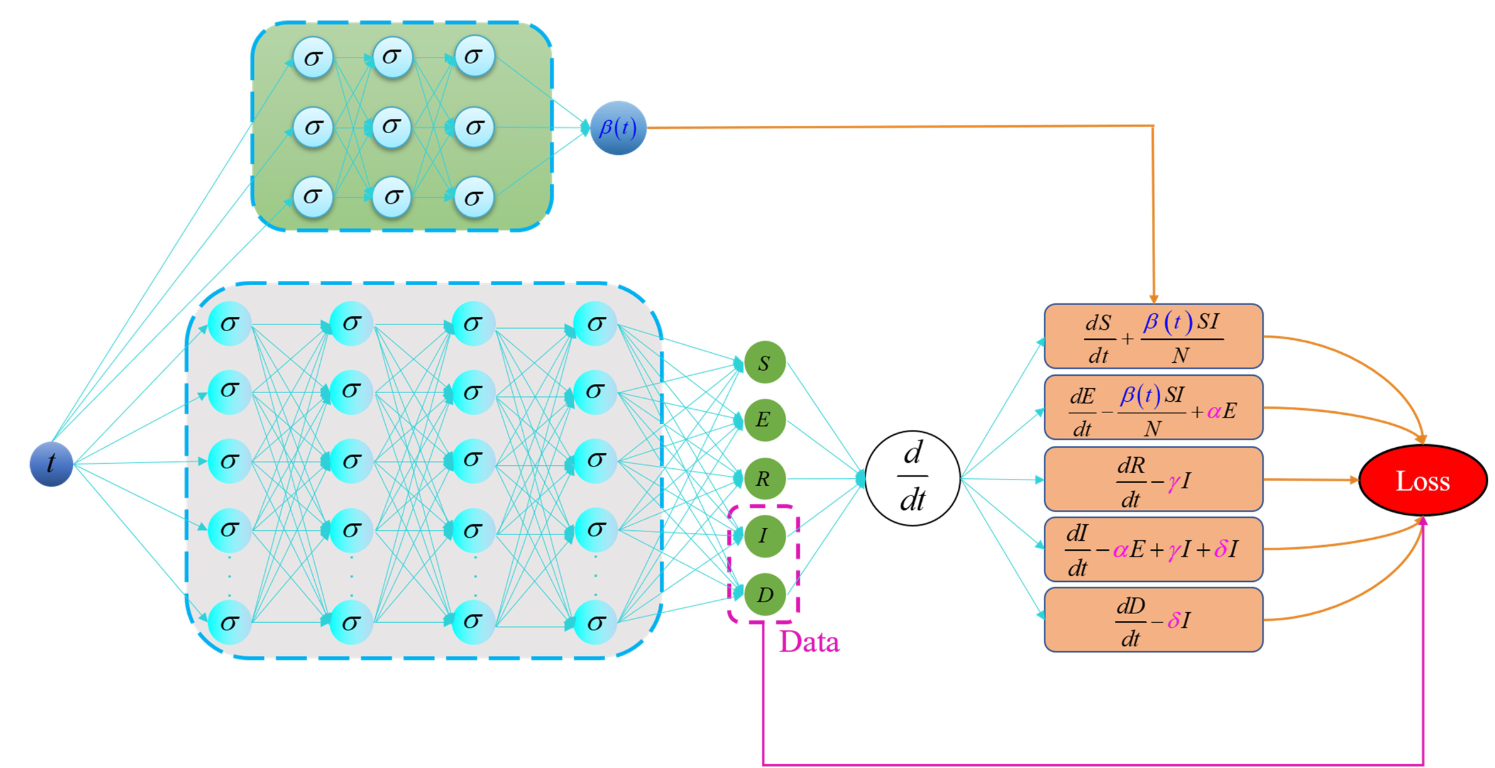
\includegraphics[width=0.8\linewidth]{img/seir.png}\label{ode-nn}
    \caption{ODE情况下理论上的网络结构}
\end{figure}
而在PDE模型\eqref{pde}中若采用两个网络则
\begin{equation}
\begin{aligned}\label{p1}
    NN_1(a,a',t)&=\lambda(a,a',t)\\
    NN_2(a,t,\lambda)&=X
\end{aligned}
\end{equation}
两个网络的输入变量不同,由以下解决方案。
\subsection{解决方案}\label{Solution}
一. 将\eqref{p1}中的$NN_2(a,t,\lambda)$增添一个输入变量$a'$变为$NN_2(a,a',t,\lambda)$

二. 化简\eqref{p1}中的$\int_{0}^{A} \lambda(a,a',t)I(a',t)da'$部分,由积分中值定理
\begin{equation}
    \int_{0}^{A} \lambda(a,a',t)I(a',t)da'=\lambda(a,\epsilon,t)\int_{0}^{A} I(a',t)da',\epsilon \in (0,A)
\end{equation}
每一对$a,t$对应一个$\epsilon$,存在$\hat{\lambda}(a,t)$
\begin{equation}
    \hat{\lambda}(a,t)=\lambda(a,\epsilon(a,t),t)
\end{equation}
可以将\eqref{p1}改为
\begin{equation}
\begin{aligned}
    NN_1(a,t)&=\hat{\lambda}(a,t)\\
    NN_2(a,t,\lambda)&=X
\end{aligned}
\end{equation}
其中$\hat{\lambda}(a,t)$的实际含义为年龄为$a$的易感群体在$t$时刻的易感程度。

三. 分布训练两个模型(预训练+LoRA微调)

在之前ode的SEIR模型\cite{he2023transmission}中,损失由数据损失和ODE损失两部分组成:
\begin{equation}
    Loss=Loss_{data}+Loss_{ODE}
\end{equation}
而在神经网络\eqref{p1}中,$NN_2(a,t)$对应$Loss_{ODE}$,可以预先设定不同的$\lambda(a,a',t)$,使用\eqref{pde}生成多组仿真数据预先训练$NN_2(a,t)$,当$NN_2(a,t)$学习到足够多的PDE信息后再将其中的参数冻结,用$NN_1(a,a',t)$代替$\lambda(a,a',t)$使用真实数据进行训练。

\begin{table}[h!]
  \begin{center}
    \caption{总结}
    \begin{tabular}{ccc} % <-- Alignments: 1st column left, 2nd middle and 3rd right, with vertical lines in between
\toprule
方案 & 优点 &不足 \\
\midrule
\multirow{2}*{一} &  1.可以得到每个年龄段对每个年龄段的传染率$\lambda(a,a',t)$ &  1.增大计算量 \\
 & 2.保持模型结构不变 & 2.现有数据量可能不足\\
\midrule
二 &  1.大幅减少计算量 &  1.只能得到每个年龄段的易感率$\lambda(a,t)$ \\
\midrule
\multirow{3}*{三} &  1.可以得到每个年龄段对每个年龄段的传染率$\lambda(a,a',t)$ &  1.增大计算量 \\
 & 2.在较少数据下表现更好 & 2.如何生成预训练的仿真数据\\
 & 3.训练好的$NN_2(a,t)$可以在其他数据集直接使用 &3. 是否具有可行性\\
\bottomrule
    \end{tabular}
  \end{center}
\end{table}

对于这三种解决方案,按照可行性从二>一>三的顺序进行。

\section{参数的问题}\label{problem}
\subsection{时间单位}
对于部分参数,师姐给出了一些文献中的参考值,如(图\ref{para})为年龄分组的数值,分组的组距为7个月、15个月、12年、5年、10年不等。同时,麻疹数据的时间单位为月,年龄单位为年(如图\ref{data}),对于本文的连续性模型应该采用怎样的时间单位?(月?年?)

如果$a$的单位为年,$t$的单位为月的话,\eqref{pde}式应改为:
\begin{equation}
  \left\{
  \begin{aligned}
  \frac{\partial}{\partial a} S(a,t)+12\frac{\partial}{\partial t} S(a,t)  =&  -(d(a,t)+(v(a,t)+\theta(a,t))p(a))S(a,t)- S(a,t)\int_{0}^{A} \lambda(a,a',t)I(a',t)da'+\delta(a) R(a,t)\\
  \frac{\partial}{\partial a} I(a,t)+12\frac{\partial}{\partial t} I(a,t)  =&  S(a,t)\int_{0}^{A} \lambda(a,a',t)I(a',t)da'-(d(a,t)+\gamma(a))I(a,t) \\
  \frac{\partial}{\partial a} R(a,t)+12\frac{\partial}{\partial t} R(a,t)  =&  (v(a,t)+\theta(a,t))p(a)S(a,t)+\gamma(a) I(a,t)-(d(a,t)+\delta(a))R(a,t)
  \end{aligned}
  \right.
\end{equation}

\begin{figure}[htbp]
  \centering
  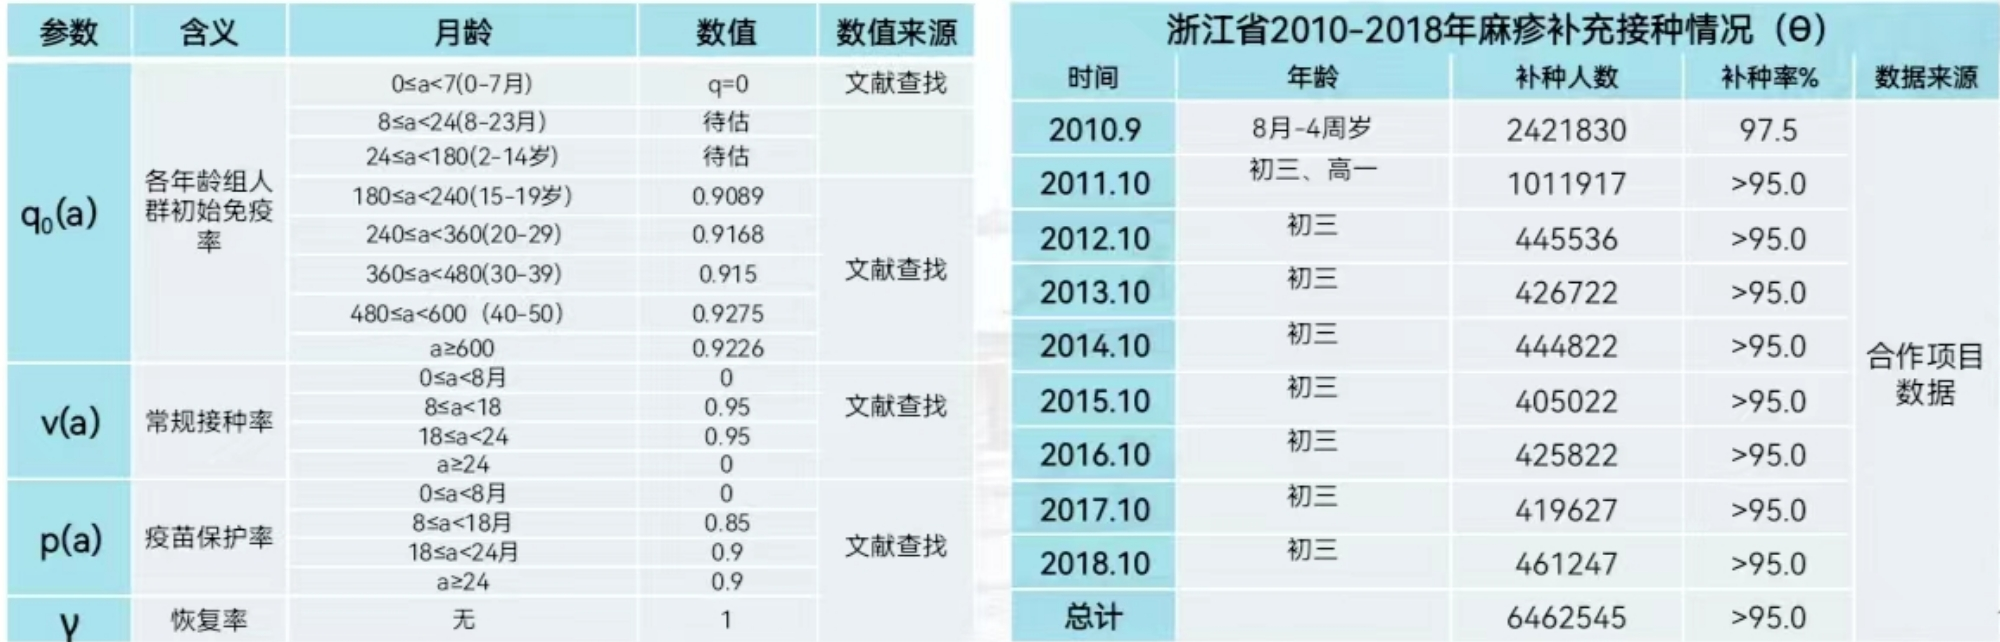
\includegraphics[width=0.8\linewidth]{img/参数.png}\label{para}
  \caption{部分参数值}
\end{figure}

\begin{figure}[htbp]
  \centering
  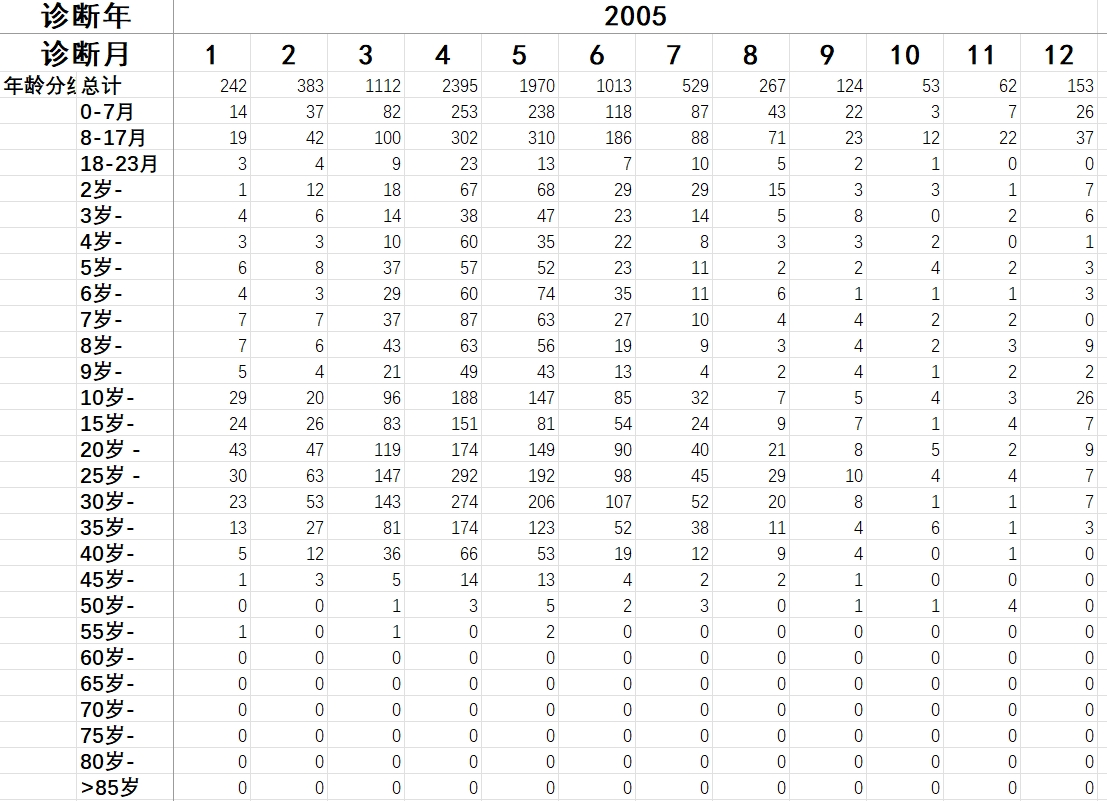
\includegraphics[width=0.8\linewidth]{img/数据分组.png}\label{data}
  \caption{麻疹数据}
\end{figure}

\subsection{差值方法的选择}
由于能够获取的参数、感染数据都是离散值,而且大部分数据点并没有相互对应。所以需要选择一种差值方法来扩充数据(部分需要二维差值方法)。可以将以下方法都试一遍选择最好的方法:

\begin{table}[h!]
  \begin{center}
    \caption{插值方法}
    \begin{tabular}{cc} % <-- Alignments: 1st column left, 2nd middle and 3rd right, with vertical lines in between
\toprule
方法 & 效果 \\
\midrule
牛顿插值 & \\
Hermite插值 & \\
三次样条插值 & \\
\bottomrule
    \end{tabular}
  \end{center}
\end{table}

\href{https://blog.csdn.net/yanfeng1022/article/details/114528323}{九种常见的二维插值方法}

\section{数据获取}
\subsection{人口年龄构成}
来源\href{https://tj.jiangsu.gov.cn/col/col89815/index.html}{江苏统计年鉴},根据分年龄段的抽样调查乘以总人数得到各年龄段的总人口。2011年数据缺失,使用2010、2012年的平均值代替。
\subsection{分年龄组死亡率}
\href{https://qikan.cqvip.com/Qikan/Article/Detail?id=7107031310}{《江苏省人口平均预期寿命估计及死因差异分析》}这篇文章数据由江苏省疾病预防控制中心提供,但在\href{https://www.jscdc.cn/xxgk_1641/}{江苏疾控官网}未找到。
\printbibliography
\end{document}
